 \documentclass[12pt]{article}
\usepackage[a4paper, margin=.30in]{geometry}

\usepackage{array}
\usepackage{graphicx, subfig, wrapfig, fancyhdr, lastpage }
\newcommand\headerMe[2]{\noindent{}#1\hfill#2}
\usepackage[mathscr]{euscript}



\pagestyle{fancy}
\fancyhf{}

\rfoot{\em{Page \thepage \hspace{1pt} / \pageref{LastPage}}}
\begin{document}

\headerMe{Royaume du Maroc}{année scolaire \emph{2022-2023}}\\
\headerMe{Ministère de l'Éducation nationale, }{  Professeur :\emph{Zakaria Haouzan}}\\
\headerMe{du Préscolaire et des Sports}{Établissement : \emph{Lycée SKHOR qualifiant}}\\

\begin{center}
Devoir  N°2 Semestre 2 \\
   Filière Tronc Commun Scientifique\\
Durée 2h00
\\
    \vspace{.2cm}
\hrulefill
\Large{Chimie 7pts/42min}
\hrulefill\\

    %\emph{Les Trois parties sont indépendantes}
\end{center}
%end Headerss------------------------
 \section*{Partie 1 :La quantité de matière et la concentration molaire \dotfill (7pts) }
On fait dissoudre une masse $m = 6,35 g$ de chlorure de fer II $(FeCl_2)$ dans l’eau pour préparer une solution $(S_1)$ de volume $V_1 = 100 mL$.

\begin{enumerate}
    \item Qu’appelle-t-on la solution $(S_1)$? \dotfill(0.5pt)
    \item Calculer la concentration massique $C_{m1}$ de la solution $(S_1)$.\dotfill(1pt)
    \item Calculer la quantité de matière du soluté $n_1$ dissout dans $(S_1)$. \dotfill(0.5pt)
    \item Calculer la concentration molaire $C_1$ de la solution $(S_1)$. \dotfill(1pt)
    \item On dispose maintenant d’une solution aqueuse $(S_2)$ de chlorure de fer II et de concentration 

		$C_2$=$0,25mol.L^{-1}$ et de volume $V_2 = 200 mL$. On mélange dans le même bêcher la solution $(S_1)$ et la solution $(S_2)$ pour obtenir une solution (S).
        \begin{enumerate}
            \item  Calculer la quantité de matière du soluté $n_2$ dissout dans $(S_2)$.\dotfill(1pt)
            \item Calculer la quantité de matière totale $n$ de soluté dissout dans la solution (S).\dotfill(1.5pt)
            \item Déduire la concentration molaire C de la solution (S).\dotfill(1pt)
            \item Déduire la concentration massique $C_m$ de la même solution (S).\dotfill(0.5pt)
        \end{enumerate}
    \end{enumerate}
\textbf{\underline{Données:} }
masses molaires en g/mol : $M(Fe) = 55,8g/mol$ ; $M(Cl)= 35,5g/mol$.
\\La masse volumique du vinaigre commercial: $\rho = 1,02 g/ml$
%__________________Chimie ______________________-
%%%%%%%+_+_+_+_+_+_+_+_+_Partie1

%_____________________________________PHYSIque Partie 22222____________________________________________________________________________
    %\vspace{2cm}
\hrulefill\\
\begin{center}
\hrulefill
\Large{Physique 13pts/72min}
\hrulefill\\
    \emph{Les deux parties sont indépendantes}
\end{center}
%end Headerss------------------------

 \section*{Partie 1 :La caractéristique d'une tension \dotfill(6 pts)}

%\begin{wrapfigure}[7]{r}{0.40\textwidth}
    %\vspace{-1cm}
    %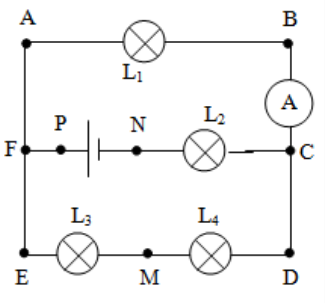
\includegraphics[width=0.36\textwidth]{./img/circuit_00.png}
%\end{wrapfigure}

On réalise deux circuits électriques dont les schémas sont représentés ci-dessous.
\begin{center}
    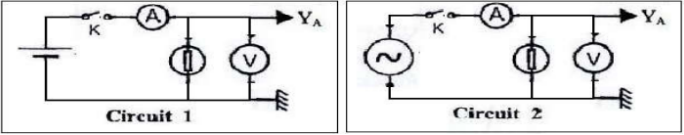
\includegraphics[width=0.5\textwidth]{./img/circuit_Ex_00.png}
\end{center}

\vspace{3cm}

\begin{enumerate}
    \item Quel est le type de la tension représentée dans  chaque oscillogramme.\dotfill(1pt)
\begin{center}
    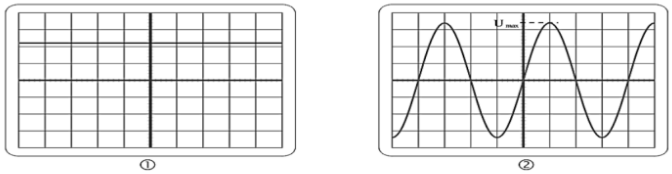
\includegraphics[width=0.8\textwidth]{./img/oscillo.png}
\end{center}
\item On se place dans le cas du circuit 2 qui a permis d’obtenir l’oscillogramme 2. La sensibilité verticale est de 5V /division.

    \begin{enumerate}
        \item Déterminer,la valeur de la tension maximale $U_{max}$.\dotfill(1pt)
        \item Le voltmètre indique une tension U. Que représente U ? calculer sa valeur.\dotfill(1pt)
        \item La sensibilité horizontale est de 5 ms/division.
            Déterminer,la période T du signal en ms puis en(s).\dotfill(2pt)
        \item En déduire la fréquence f du signal.\dotfill(1pt)
    \end{enumerate}
\end{enumerate}


\hrulefill\\
%_________________partie 2  : gravitation universelle :)
\section*{Partie 2 : La Mesure de l’intensité du courant éléctrique: \dotfill(7pts)}

\begin{wrapfigure}[6]{r}{0.40\textwidth}
    \vspace{-1cm}
\begin{center}
    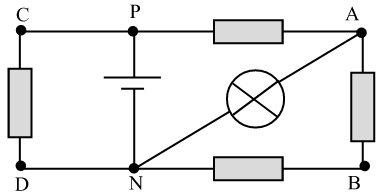
\includegraphics[width=0.36\textwidth]{./img/circuit_01.png}
\end{center}
    \end{wrapfigure}
On réalise le montage de la figure ci-contre.
\begin{enumerate}
    \item Indiquer le sens des différents courants électriques dans les
        branches du circuit.\dotfill(2pt)
    \item Compléter le tableau des intensités.\dotfill(2pt)
          \begin{tabular}{ | l | l | l | l |l|l|l|l|l|}
    \hline
              Branche       & NP & PA & AB & BN & PC & CD & DN & AN  \\\hline
              Intensité (A) & 3   &    &    & 0.5   &    &  &1       &       \\ \hline
    \end{tabular}
\item Compléter les tableaux suivants (C : Calibre ; 
n : nombre de division indiqué par l’aiguille ; $n_0$  : nombre de division de cadran)\dotfill(3pt)
\begin{center}
    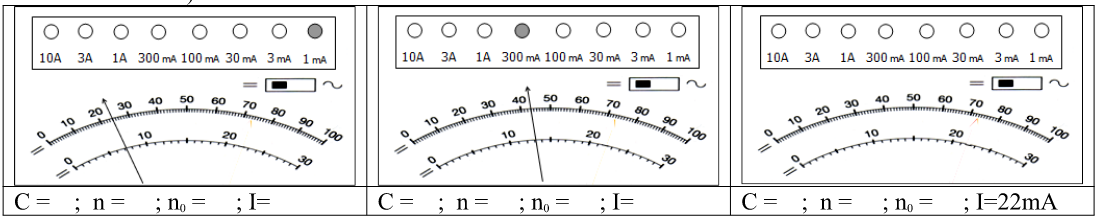
\includegraphics[width=0.95\textwidth]{./img/circuit_03.png}
\end{center}

\end{enumerate}
%\begin{wrapfigure}[3]{r}{0.40\textwidth}
    %\vspace{-1cm}

    %\end{wrapfigure}
\end{document}
